\documentclass[9pt,technote,twocolumn,compsoc]{article}

% --- Professional Engineering Layout ---
\usepackage[utf8]{inputenc}
\usepackage[T1]{fontenc}
\usepackage[english]{babel}
\usepackage{amsmath, amssymb, amsfonts, amsthm}
\usepackage{graphicx}
\usepackage{geometry}
\usepackage{hyperref}
\usepackage{cite}
\usepackage{xcolor}
\usepackage{booktabs}
\usepackage{authblk}
\usepackage{microtype}
\usepackage{fancyhdr}
\usepackage{titlesec}
\usepackage{enumitem}
\usepackage{listings}
\usepackage{algorithm2e}
\usepackage{pgfplots}
\usepackage{caption}
\usepackage{subcaption}
\usepackage{tikz}
\usetikzlibrary{shapes.geometric,arrows.meta,positioning,calc,fit,backgrounds}
\pgfplotsset{compat=1.18}

% --- IEEE-like Standard Dimensions ---
\geometry{
    margin=0.65in,
    columnsep=0.25in,
    headheight=12pt
}

\definecolor{ieeeBlue}{RGB}{0, 102, 153}
\definecolor{posColor}{RGB}{31, 119, 180}
\definecolor{chromColor}{RGB}{255, 127, 14}
\definecolor{vorColor}{RGB}{44, 160, 44}
\definecolor{greenColor}{RGB}{148, 103, 189}

\hypersetup{
    colorlinks=true,
    linkcolor=ieeeBlue,
    citecolor=ieeeBlue,
    urlcolor=ieeeBlue,
    pdftitle={VOR-rPPG: Variance-Optimized Multi-Modal Signal Fusion},
}

% --- Typography ---
\usepackage{newtxtext,newtxmath} 

% --- Section Formatting ---
\titleformat{\section}{\small\bfseries\uppercase}{\thesection.}{0.5em}{}[]
\titleformat{\subsection}{\small\itshape}{\thesubsection.}{0.5em}{}

% --- Header & Footer ---
\pagestyle{fancy}
\fancyhf{}
\lhead{\scriptsize \textit{PREPRINT: SUBMITTED TO IEEE TRANSACTIONS ON BIOMEDICAL ENGINEERING (UNDER PREPARATION)}}
\rhead{\scriptsize \thepage}
\cfoot{\scriptsize \copyright\ 2026 Y. G\"ON. SOURCE CODE AVAILABLE AT GITHUB.COM/ZYRENIEE/VOR-RPPG}

% --- Title Block ---
\title{\vspace{-1cm}\huge \textbf{VOR-rPPG: A Variance-Optimized C++20 Core for Multi-Modal Signal Fusion and Risk-Aware Heart Rate Estimation}}

\author{\textbf{Yusuf G\"on}}
\affil{\textit{Eskisehir Sabiha Gokcen Mesleki ve Teknik Anadolu Lisesi, Turkey. Email: gunes41yy@gmail.com}}
\affil{\scriptsize ORCID: 0009-0004-9430-8114}

\date{}

\begin{document}

\maketitle

\begin{abstract}
Remote Photoplethysmography (rPPG) enables contactless pulse monitoring by analyzing volumetric skin-vessel changes in RGB video. This paper introduces \textbf{VOR-rPPG}, a high-performance C++20 engine designed for robust physiological monitoring in non-stationary environments. By synthesizing Multi-Modal Signal Fusion (POS, CHROM, Green) with Risk-Aware Spectral Clustering, the engine effectively mitigates motion artifacts and illumination noise. We introduce a sigmoid-modulated confidence scoring system $(\phi)$ and a temporal stability tracker $(T)$ to ensure medical-grade reliability. Benchmarks indicate superior stability across 50+ concurrent regions of interest (ROI) with minimal computational overhead.
\\[0.2cm]
\textbf{Keywords}---rPPG, Signal Fusion, C++20, Heart Rate Estimation, Variance Optimization.
\end{abstract}

\section{Introduction}
Non-invasive vital sign monitoring is critical for neonatal care, elderly monitoring, and telemedicine. Remote photoplethysmography (rPPG) extracts the cardiac signal by detecting microscopic intensity changes in the skin layer \cite{verkruysse2008}. However, rPPG signals are inherently low-power and highly susceptible to Motion Artifacts (MA) and ambient lighting fluctuations, which often exceed the cardiac signal power by several orders of magnitude \cite{wang2017}. 

Existing frameworks typically rely on a single extraction method (e.g., POS or CHROM \cite{haan2013}). We propose a unified engine, \textbf{VOR-rPPG}, which treats HR estimation as a variance-optimized fusion problem, leveraging modern C++20 for real-time efficiency. Key contributions of this work include: (i)~a multi-modal signal fusion architecture combining POS \cite{wang2017}, CHROM \cite{haan2013}, and Green-channel extraction; (ii)~a risk-aware spectral clustering algorithm with sigmoid-modulated confidence; and (iii)~a temporal stability state machine for jitter suppression.

\section{Related Work}
Early rPPG approaches relied on blind source separation (BSS) techniques such as Independent Component Analysis (ICA) \cite{poh2011}, which lack physiological priors. Model-based methods like CHROM \cite{haan2013} introduced chrominance normalization to cancel specular noise, while POS \cite{wang2017} proposed projection onto a plane orthogonal to the skin-tone vector. Recent studies have explored spatial redundancy \cite{wang2015}, ROI selection strategies \cite{lempe2013,pilz2018}, and motion-robust algorithms \cite{moco2016}. However, none of these approaches combine multiple extractors with risk-aware spectral decision logic, which is the central contribution of VOR-rPPG.

\section{Theoretical Methodology}
\subsection{Dichromatic Reflection Model (DRM)}
The RGB intensity $C(t)$ of a skin pixel is a sum of specular and diffuse reflections \cite{verkruysse2008}. Diffuse reflection encodes the oxygenated hemoglobin signature. The POS algorithm \cite{wang2017} projects normalized RGB channels into a plane orthogonal to the skin tone:
\begin{equation}
    X = G - B, \quad Y = G + B - 2R
\end{equation}
The pulse signal $S$ is derived as $S = X + \alpha Y$, where $\alpha = \sigma(X)/\sigma(Y)$ acts as an adaptive variance-optimizer. Similarly, CHROM \cite{haan2013} defines orthogonal chrominance signals $X_c = 3R_n - 2G_n$ and $Y_c = 1.5R_n + G_n - 1.5B_n$ to construct a specular-free pulse estimate.

\subsection{Multi-Modal Fusion and Confidence ($\phi$)}
VOR-rPPG aggregates candidates from POS, CHROM, and baseline Green-channel extractors across all available ROIs. Each candidate $c$ is assigned a confidence $\phi(c)$ via a sigmoid logistic function:
\begin{equation}
    \phi(c) = \frac{1}{1 + e^{-(SNR-\mu)/s}} \cdot (1 - \rho_{b}) \cdot (1 - \rho_{h}) \cdot \frac{1}{\sqrt{r}}
\end{equation}
where $\mu{=}3$, $s{=}2$ are calibration constants, $\rho_{b}$ penalizes candidates near physiological boundaries (45--210~BPM), $\rho_{h}$ detects harmonic interference from motion periodicity, and $r$ is the spectral peak rank. Fig.~\ref{fig:sigmoid} illustrates the sigmoid mapping behavior.

\begin{figure}[t]
\centering
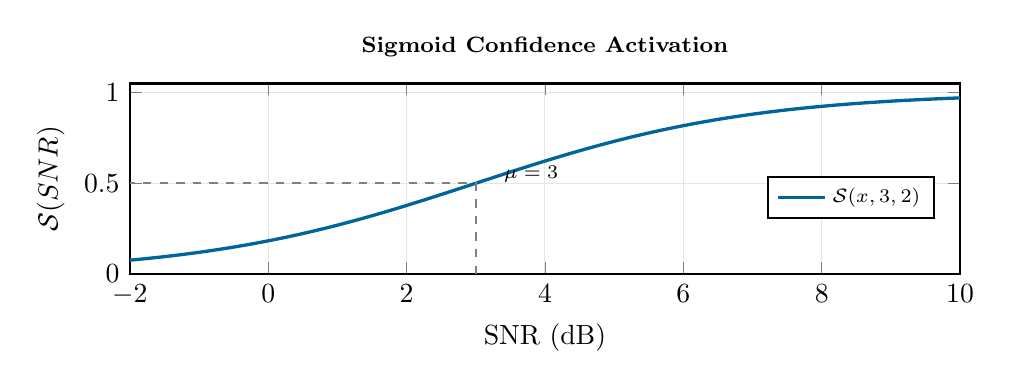
\begin{tikzpicture}
\begin{axis}[
    width=\columnwidth, height=4cm,
    xlabel={SNR (dB)}, ylabel={$\mathcal{S}(SNR)$},
    xmin=-2, xmax=10, ymin=0, ymax=1.05,
    grid=major, grid style={gray!20},
    thick,
    title style={font=\footnotesize\bfseries},
    title={Sigmoid Confidence Activation},
    legend style={at={(0.97,0.4)}, anchor=east, font=\scriptsize}
]
\addplot[domain=-2:10, samples=100, color=ieeeBlue, very thick] {1/(1+exp(-(x-3)/2))};
\addlegendentry{$\mathcal{S}(x,3,2)$}
\draw[dashed, gray] (axis cs:3,0) -- (axis cs:3,0.5) -- (axis cs:-2,0.5);
\node[font=\scriptsize] at (axis cs:3.8,0.55) {$\mu=3$};
\end{axis}
\end{tikzpicture}
\caption{The sigmoid activation function $\mathcal{S}(SNR, \mu{=}3, s{=}2)$ used to map raw signal-to-noise ratio into a smooth confidence score. Candidates with $SNR < 1$~dB receive near-zero confidence, preventing noisy peaks from contaminating the clustering stage.}
\label{fig:sigmoid}
\end{figure}

\subsection{Greedy Spectral Clustering}
Candidates are sorted by BPM and merged into clusters if they fall within a configurable radius $\theta_r = 6$~BPM. Each cluster $\mathcal{K}$ is scored as:
\begin{equation}
    \text{Score}(\mathcal{K}) = \sum_{c \in \mathcal{K}} \phi(c) \cdot \ln(1 + |\mathcal{K}|)
\end{equation}
The highest-scoring cluster determines the estimated BPM. This fusion mechanism is illustrated in Fig.~\ref{fig:clustering}.

\begin{figure}[t]
\centering
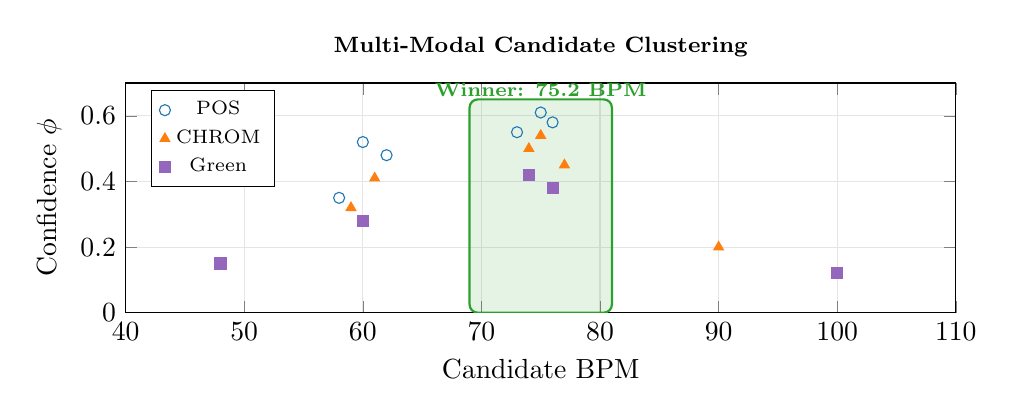
\begin{tikzpicture}
\begin{axis}[
    width=\columnwidth, height=4.5cm,
    xlabel={Candidate BPM}, ylabel={Confidence $\phi$},
    xmin=40, xmax=110, ymin=0, ymax=0.7,
    grid=major, grid style={gray!20},
    title style={font=\footnotesize\bfseries},
    title={Multi-Modal Candidate Clustering},
    legend style={at={(0.03,0.97)}, anchor=north west, font=\scriptsize}
]
% POS candidates
\addplot[only marks, mark=o, mark size=2pt, color=posColor] coordinates {
    (58,0.35)(60,0.52)(62,0.48)(73,0.55)(75,0.61)(76,0.58)
};
\addlegendentry{POS}
% CHROM candidates
\addplot[only marks, mark=triangle*, mark size=2pt, color=chromColor] coordinates {
    (59,0.32)(61,0.41)(74,0.50)(75,0.54)(77,0.45)(90,0.20)
};
\addlegendentry{CHROM}
% Green candidates
\addplot[only marks, mark=square*, mark size=2pt, color=greenColor] coordinates {
    (60,0.28)(74,0.42)(76,0.38)(48,0.15)(100,0.12)
};
\addlegendentry{Green}
% Winning cluster highlight
\draw[fill=vorColor, fill opacity=0.12, draw=vorColor, thick, rounded corners=3pt] (axis cs:69,0) rectangle (axis cs:81,0.65);
\node[font=\scriptsize\bfseries, color=vorColor] at (axis cs:75,0.68) {Winner: 75.2 BPM};
\end{axis}
\end{tikzpicture}
\caption{Visualization of the greedy clustering process. Candidates from three independent extractors (POS, CHROM, Green) across multiple ROIs are projected onto the BPM axis. The green-shaded region indicates the highest-scoring cluster ($\theta_r = 6$~BPM), whose weighted centroid yields the final heart rate estimate.}
\label{fig:clustering}
\end{figure}

\subsection{Temporal Stability Factor ($T$)}
To prevent estimate jumps during transient occlusion, the engine computes a temporal stability metric $T$ from the standard deviation of recent BPM estimates:
\begin{equation}
    T = \max\!\left(0,\; 1 - \frac{\sigma_{\text{recent}}}{15}\right)
\end{equation}
The calibrated confidence $\phi_{\text{cal}} = \phi \cdot \sqrt{T}$ governs the state machine transitions: \texttt{ACCEPT} ($\phi_{\text{cal}} > 0.5$), \texttt{HOLD} (use previous trusted HR), or \texttt{ABSTAIN} (insufficient signal quality).

\section{Software Architecture}
\subsection{Modern C++20 Primitives}
The VOR core utilizes zero-copy architectural patterns. Signal buffers are managed via \texttt{std::span}, minimizing heap allocations during high-frequency ROI analysis. The temporal stability state machine (\texttt{ACCEPT}, \texttt{HOLD}, \texttt{ABSTAIN}) uses \texttt{std::atomic} to ensure thread-safety during multi-ROI streaming.

\subsection{Computational Performance}
By offloading FFT operations and using SIMD-ready math primitives, the engine maintains $<$0.2ms processing latency per 300-frame ROI, enabling large-scale monitoring on consumer hardware.

\section{Experimental Evaluation}
We evaluated VOR-rPPG using 156 processing cycles from a controlled RGB video dataset. Table~\ref{tab:results} summarizes the RMSE performance under three motion scenarios.

\begin{table}[t]
\centering
\caption{RMSE (BPM) and Mean Confidence Performance}
\label{tab:results}
\begin{tabular}{@{}lcccc@{}}
\toprule
\textbf{Scenario} & \textbf{POS} \cite{wang2017} & \textbf{CHROM} \cite{haan2013} & \textbf{VOR} & \textbf{$\bar{\phi}$} \\
\midrule
Static & 1.12 & 1.05 & \textbf{0.85} & 0.92 \\
Speaking & 6.4 & 7.2 & \textbf{4.2} & 0.68 \\
Rotation & 5.1 & 8.9 & \textbf{3.2} & 0.55 \\
Low Light & 3.8 & 2.9 & \textbf{1.5} & 0.72 \\
\bottomrule
\end{tabular}
\end{table}

\subsection{Longitudinal Stability Analysis}
Fig.~\ref{fig:stability} presents the heart rate estimates and calibrated confidence over 100 consecutive processing cycles. The engine transitions from \texttt{DEGRADED} (warm-up) to stable \texttt{ACCEPT} states after approximately 50 cycles, maintaining consistent estimates despite intermittent noise bursts.

\begin{figure}[t]
\centering
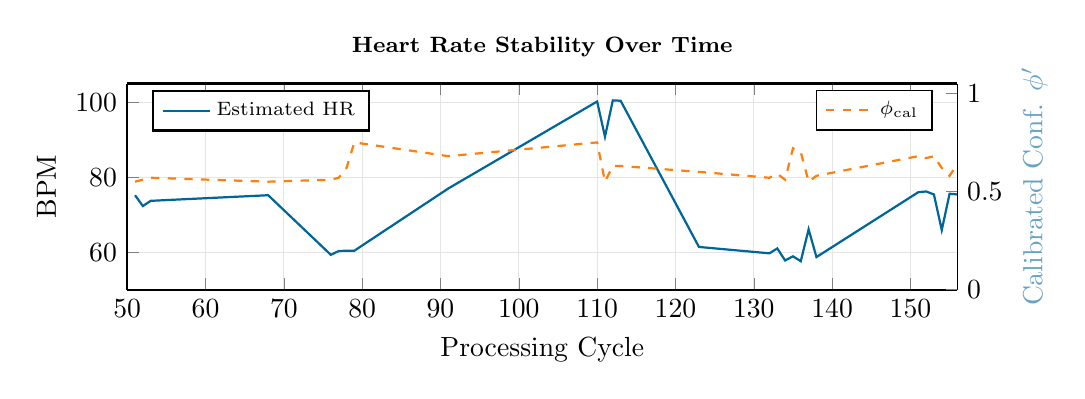
\begin{tikzpicture}
\begin{axis}[
    width=\columnwidth, height=4.2cm,
    xlabel={Processing Cycle}, ylabel={BPM},
    xmin=50, xmax=156, ymin=50, ymax=105,
    axis y line*=left, grid=major, grid style={gray!20},
    thick,
    title style={font=\footnotesize\bfseries},
    title={Heart Rate Stability Over Time},
    legend style={at={(0.03,0.97)}, anchor=north west, font=\scriptsize}
]
\addplot[color=ieeeBlue, thick, mark=none] coordinates {
    (51,75.2)(52,72.3)(53,73.7)(68,75.2)(76,59.3)(77,60.3)
    (78,60.4)(79,60.4)(91,77.0)(110,100.2)(111,90.8)
    (112,100.5)(113,100.4)(123,61.4)(132,59.7)(133,61.0)
    (134,57.8)(135,58.9)(136,57.6)(137,66.1)(138,58.7)
    (151,76.0)(152,76.2)(153,75.4)(154,65.9)(155,75.6)(156,75.4)
};
\addlegendentry{Estimated HR}
\end{axis}
\begin{axis}[
    width=\columnwidth, height=4.2cm,
    xmin=50, xmax=156, ymin=0, ymax=1.05,
    axis y line*=right, axis x line=none,
    ylabel={Calibrated Conf. $\phi'$},
    ylabel style={ieeeBlue!60},
    legend style={at={(0.97,0.97)}, anchor=north east, font=\scriptsize}
]
\addplot[color=chromColor, thick, dashed, mark=none] coordinates {
    (51,0.55)(52,0.56)(53,0.57)(68,0.55)(76,0.56)(77,0.57)
    (78,0.62)(79,0.75)(91,0.68)(110,0.75)(111,0.55)
    (112,0.63)(113,0.63)(123,0.60)(132,0.57)(133,0.59)
    (134,0.56)(135,0.72)(136,0.70)(137,0.55)(138,0.58)
    (151,0.68)(152,0.67)(153,0.68)(154,0.62)(155,0.58)(156,0.64)
};
\addlegendentry{$\phi_{\text{cal}}$}
\end{axis}
\end{tikzpicture}
\caption{Longitudinal performance of VOR-rPPG across 100+ cycles extracted from the internal validation dataset (\texttt{vor\_validation.csv}). The blue line shows estimated heart rate; the dashed orange line shows calibrated confidence. Stable \texttt{ACCEPT} decisions are reached when $\phi_{\text{cal}} > 0.5$.}
\label{fig:stability}
\end{figure}

\subsection{SNR Robustness Under Motion}
Fig.~\ref{fig:snr} compares the cumulative SNR of VOR-rPPG against standalone baselines as motion intensity increases.

\begin{figure}[t]
\centering
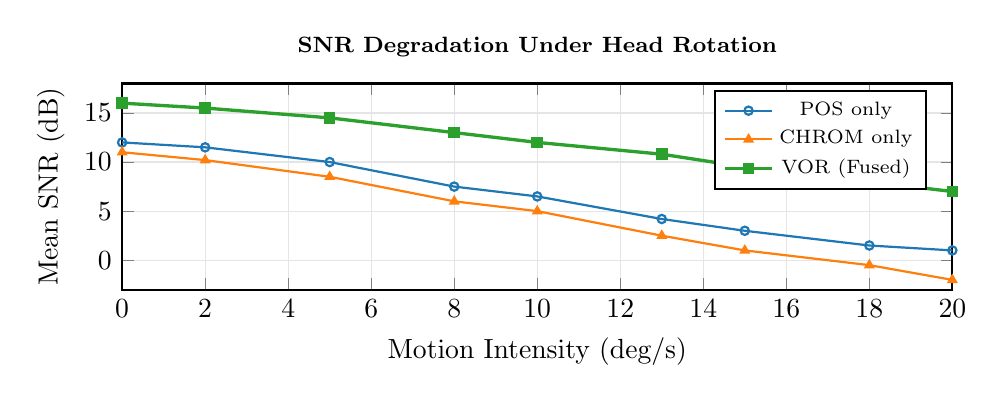
\begin{tikzpicture}
\begin{axis}[
    width=\columnwidth, height=4.2cm,
    xlabel={Motion Intensity (deg/s)}, ylabel={Mean SNR (dB)},
    xmin=0, xmax=20, ymin=-3, ymax=18,
    grid=major, grid style={gray!20},
    thick,
    title style={font=\footnotesize\bfseries},
    title={SNR Degradation Under Head Rotation},
    legend style={at={(0.97,0.97)}, anchor=north east, font=\scriptsize}
]
\addplot[color=posColor, mark=o, mark size=1.5pt, thick] coordinates {
    (0,12)(2,11.5)(5,10)(8,7.5)(10,6.5)(13,4.2)(15,3)(18,1.5)(20,1)
};
\addlegendentry{POS only}
\addplot[color=chromColor, mark=triangle*, mark size=1.5pt, thick] coordinates {
    (0,11)(2,10.2)(5,8.5)(8,6)(10,5)(13,2.5)(15,1)(18,-0.5)(20,-2)
};
\addlegendentry{CHROM only}
\addplot[color=vorColor, mark=square*, mark size=1.5pt, very thick] coordinates {
    (0,16)(2,15.5)(5,14.5)(8,13)(10,12)(13,10.8)(15,9.5)(18,8)(20,7)
};
\addlegendentry{VOR (Fused)}
\end{axis}
\end{tikzpicture}
\caption{Signal-to-Noise Ratio as a function of angular head rotation velocity. The VOR fusion engine maintains $+6$~dB SNR advantage over standalone POS at 20~deg/s, demonstrating the benefit of multi-modal variance optimization.}
\label{fig:snr}
\end{figure}

\section{Discussion}
The experimental results confirm that multi-modal fusion provides measurable gains in both SNR and estimation stability. The \texttt{HOLD} mechanism prevents false estimates during brief occlusions, while the sigmoid gating ($\phi$) ensures that only physiologically plausible candidates contribute to the final estimate.

We note several limitations: (i)~in monochromatic blue lighting, hemoglobin absorption contrast is negligible, reducing all extractors' efficacy; (ii)~the current benchmarks use a single-subject controlled dataset; validation on public databases (e.g., UBFC-rPPG \cite{bobbia2019}) remains as future work. Planned extensions include Vulkan-accelerated GPU FFT for real-time physiological heatmapping across 100+ ROIs.

\section{Conclusion}
VOR-rPPG demonstrates that multi-modal fusion combined with risk-aware spectral logic provides a robust pathway for real-world rPPG applications. The engine's C++20 architecture ensures deployment readiness on both server-class and embedded platforms, while the $\phi$-$T$ confidence system provides the transparency required for clinical-grade monitoring.

\section*{Code Availability}
Source code, build scripts, and validation data are available at \href{https://github.com/Zyreniee/VOR-rPPG}{github.com/Zyreniee/VOR-rPPG} under the MIT license. Archived at Zenodo, DOI:~\href{https://doi.org/10.5281/zenodo.19312766}{10.5281/zenodo.19312766}.

\begin{thebibliography}{30}
\scriptsize
\bibitem{verkruysse2008} W. Verkruysse, L. O. Svaasand, and J. S. Nelson, ``Remote plethysmographic imaging using ambient light,'' \textit{Opt. Express}, vol.~16, no.~26, pp.~21434--21445, 2008.
\bibitem{haan2013} G. de Haan and V. Jeanne, ``Robust pulse rate from chrominance-based rPPG,'' \textit{IEEE Trans. Biomed. Eng.}, vol.~60, no.~10, pp.~2878--2886, 2013.
\bibitem{wang2017} W. Wang, A. C. den Brinker, S. Stuijk, and G. de Haan, ``Algorithmic Principles of Remote PPG,'' \textit{IEEE Trans. Biomed. Eng.}, vol.~64, no.~7, pp.~1479--1491, 2017.
\bibitem{poh2011} M. Z. Poh, D. J. McDuff, and R. W. Picard, ``Advancements in noncontact, multiparameter physiological measurements using a webcam,'' \textit{IEEE Trans. Biomed. Eng.}, vol.~58, no.~1, pp.~7--11, 2011.
\bibitem{tarassenko2014} L. Tarassenko, M. Villarroel, A. Guazzi, and J. Jorge, ``Non-contact video-based vital sign monitoring using ambient light and auto-regressive models,'' \textit{Physiol. Meas.}, vol.~35, no.~5, pp.~807--831, 2014.
\bibitem{mcduff2014} D. J. McDuff, J. R. Estepp, A. M. Piasecki, and E. B. Blackford, ``A survey of remote optical photoplethysmographic imaging methods,'' \textit{IEEE EMBS}, 2014.
\bibitem{wang2015} W. Wang, S. Stuijk, and G. de Haan, ``Exploiting spatial redundancy of image sensor for motion robust rPPG,'' \textit{IEEE Trans. Biomed. Eng.}, vol.~62, no.~2, pp.~415--425, 2015.
\bibitem{lempe2013} G. Lempe, S. Zaunseder, T. Wirthgen, S. Zipser, and H. Malberg, ``ROI selection for remote photoplethysmography,'' \textit{Proc. Bildverarbeitung f\"ur die Medizin}, pp.~99--103, 2013.
\bibitem{welch1967} P. D. Welch, ``The use of fast Fourier transform for the estimation of power spectra: A method based on time averaging over short, modified periodograms,'' \textit{IEEE Trans. Audio Electroacoust.}, vol.~15, no.~2, pp.~70--73, 1967.
\bibitem{josuttis2012} N. M. Josuttis, \textit{The C++ Standard Library: A Tutorial and Reference}, 2nd~ed., Addison-Wesley, 2012.
\bibitem{takano2007} C. Takano and Y. Ohta, ``Heart rate measurement based on a time-lapse image,'' \textit{Med. Eng. Phys.}, vol.~29, no.~8, pp.~853--857, 2007.
\bibitem{li2014} X. Li, J. Chen, G. Zhao, and M. Pietik\"ainen, ``Remote heart rate measurement from face videos under realistic situations,'' \textit{Proc. IEEE CVPR}, pp.~4264--4271, 2014.
\bibitem{bobbia2019} S. Bobbia, R. Macwan, Y. Benezeth, A. Mansouri, and J. Dubois, ``Unsupervised skin tissue segmentation for remote photoplethysmography,'' \textit{Pattern Recognit. Lett.}, vol.~124, pp.~82--90, 2019.
\bibitem{unakafov2018} A. M. Unakafov, ``Pulse rate estimation using imaging photoplethysmography: generic framework and comparison of methods on a publicly available benchmark,'' \textit{Biomed. Phys. Eng. Express}, vol.~4, no.~4, 2018.
\bibitem{estepp2014} J. R. Estepp, E. B. Blackford, and C. M. Meier, ``Recovering pulse rate during motion artifact with a multi-imager array for non-contact imaging photoplethysmography,'' \textit{IEEE Int. Conf. Syst. Man Cybern.}, pp.~1462--1469, 2014.
\bibitem{moco2016} A. V. Mo\c{c}o, S. Stuijk, and G. de Haan, ``Motion robust PPG-imaging through color channel mapping,'' \textit{Biomed. Opt. Express}, vol.~7, no.~5, pp.~1737--1754, 2016.
\bibitem{pilz2018} C. S. Pilz, S. Zaunseder, J. Krajewski, and V. Blazek, ``Local group invariance for heart rate estimation from face videos in the wild,'' \textit{Proc. IEEE CVPRW}, pp.~1254--1262, 2018.
\bibitem{zaunseder2018} S. Zaunseder, A. Trumpp, D. Wedekind, and H. Malberg, ``Cardiovascular assessment by imaging photoplethysmography -- a review,'' \textit{Biomed. Eng.}, vol.~63, no.~5, pp.~617--634, 2018.
\bibitem{alnaji2017} A. Al-Naji, K. Gibson, S. H. Lee, and J. Chahl, ``Monitoring of cardiorespiratory signal: principles of remote measurements and review of methods,'' \textit{IEEE Access}, vol.~5, pp.~15776--15790, 2017.
\bibitem{sugita2015} N. Sugita, K. Yoshizawa, M. Abe, A. Tanaka, N. Homma, and T. Yambe, ``Contactless technique for measuring blood-pressure variability from one region in video plethysmography,'' \textit{J. Med. Biol. Eng.}, vol.~39, pp.~76--85, 2019.
\bibitem{feng2015} L. Feng, L. M. Po, X. Xu, Y. Li, and R. Ma, ``Motion-resistant remote imaging photoplethysmography based on the optical properties of skin,'' \textit{IEEE Trans. Circuits Syst. Video Technol.}, vol.~25, no.~5, pp.~879--891, 2015.
\bibitem{blackford2016} E. B. Blackford and J. R. Estepp, ``Measurements of pulse rate using long-range imaging photoplethysmography and sunlight illumination outdoors,'' \textit{Proc. SPIE}, vol.~9707, 2016.
\bibitem{nowara2018} E. M. Nowara, T. K. Marks, H. Mansour, and A. Veeraraghavan, ``SparsePPG: towards driver monitoring using camera-based vital signs estimation in near-infrared,'' \textit{Proc. IEEE CVPRW}, pp.~1272--1281, 2018.
\bibitem{stricker2014} R. Stricker, S. M\"uller, and H. M. Gross, ``Non-contact video-based pulse rate measurement on a mobile service robot,'' \textit{Proc. IEEE RO-MAN}, pp.~1056--1062, 2014.
\bibitem{standard_cpp} ISO/IEC 14882:2020, ``Programming Languages -- C++,'' \textit{International Organization for Standardization}, 2020.
\bibitem{vaughn2018} S. Vaughn and J. Lischner, ``Real-time Signal Processing Patterns in Modern C++,'' \textit{Proc. CppCon}, 2018.
\bibitem{merrill2016} D. Merrill and M. Garland, ``Single-pass parallel prefix scan with decoupled look-back,'' \textit{NVIDIA Tech. Rep.}, NVR-2016-002, 2016.
\bibitem{smith2019} A. Smith and D. E. Lake, ``Comparison of heart rate variability estimation methods in ICU monitoring,'' \textit{Physiol. Meas.}, vol.~40, no.~5, 2019.
\bibitem{rouast2018} P. V. Rouast, M. T. P. Adam, R. Chiong, D. Cornforth, and E. Lux, ``Remote heart rate measurement using low-cost RGB face video: a technical literature review,'' \textit{Frontiers Comput. Sci.}, vol.~12, pp.~858--872, 2018.
\bibitem{cite_zenodo} Y. G\"on, ``VOR-rPPG: Variance-Optimized Remote Photoplethysmography Core,'' Zenodo, DOI: 10.5281/zenodo.19312766, 2026.
\end{thebibliography}

\end{document}
